\documentclass[../main.tex]{subfiles}

\begin{document}
	\section{Dynamics}
		\begin{preamb}
			In physics, forces change the state of motion of an object. Studying forces allow us to talk about the effects on the object and predict the motions of the object. In this chapter, we will look at two-dimensional dynamics.                         
		\end{preamb}
	
		\subsection{Forces}
		\pdef{Force}{A force is a push or pull on a body. The SI unit of force is the newton [\si{\newton}].}
		
		\subsection{Newton's Laws of Motion}
		The three laws of motion are:
		\pdef{First Law}{Newton's first law states that every object will continue in its state of rest or uniform motion in a straight line unless a resultant force acts on it.}
		\pdef{Second Law}{Newton's second law states that when a resultant force acts on an object of a constant mass, the object will accelerate in the direct ion of the resultant force. The product of the mass \(m\) and acceleration \(a_{\mathrm{net}}\) of the object gives the resultant force. \[F_{\mathrm{net}} = ma_{\mathrm{net}}\]}
		\pdef{Third Law}{Newton's third law states that if body A exerts a force \(F_{AB}\) on body B, body B will exert an equal and opposite force \(F_{BA}\) on body A.}
		
		\subsection{Effects of Forces}
		From the first law, we know that a force can accelerate a body (\textit{i.e.} change velocity). This can be done by either changing the magnitude or direction of the velocity vector of the body.
			
		\subsubsection{Static System}
		\pdef{Equilibrium}{A body is said to be in equilibrium if the net force on the body is zero. This is sometimes called a static system, where no net acceleration takes place.}
			
		When resolving statics problems, it is important to ensure all force vectors add up to zero. Graphically, all these vectors when placed tip to tail should end where they started.
			
		\subsubsection{Unbalanced System}
		If the net force on a body is not zero, the object is not in translational equilibrium, and that means its velocity is changing.
			
		
		\subsection{Types of Forces}
		It is not sufficient to just describe forces as ``push'' and ``pull'' forces. Different names for forces are designated for different contexts. In this syllabus, only friction is required, but I will add common forces as well. Refer to chapter 4 for weight.
		
			\subsubsection{Normal Force}
			\pdef{Normal Force}{The normal force is the force perpendicular to a surface that the surface applies to a body due to its compression.}
			\begin{center}
				\begin{tikzpicture}
					\draw (2,0) -- (2,1) -- (3,1) -- (3,0);
					\draw [line width=0.5mm, -stealth] (2.5,0.5) -- (2.5,-1.5) node[anchor=north] {\(mg\)};
					\draw [line width=0.5mm, -stealth] (2.6,0) -- (2.6,2) node[anchor=south] {\(N\)};
					\draw (0,0) -- (5,0) node[pos=1.0, anchor=north east] {surface};
				\end{tikzpicture}
			\end{center}
		
			\subsubsection{Tension}
			\pdef{Tension}{Tension is the force exerted in a body when it is pulled on.}
			On a massless string, the tension on the two ends are equal.
			\begin{center}
				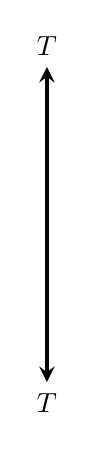
\begin{tikzpicture}
					\draw [line width=0.5mm, stealth-] (0,2) node[anchor=south] {\(T\)} -- (0,0) ;
					\draw [line width=0.5mm, -stealth] (0,0) -- (0,-2) node[anchor=north] {\(T\)};
				\end{tikzpicture}
			\end{center}
		
			\subsubsection{Friction}
			\pdef{Friction}{is the contact force that opposes or tends to oppose motion between surfaces in contact.}
			Friction is a resistive force, that works against a force applied. There are two types of friction: kinetic and static friction. 
			
			Kinetic friction deals with two objects moving on each other, and exists when an object is moving, while static friction deals with two objects that are stationary. The maximum static friction is the minimum force to be applied to allow an object to start moving on a surface.
			\begin{center}
				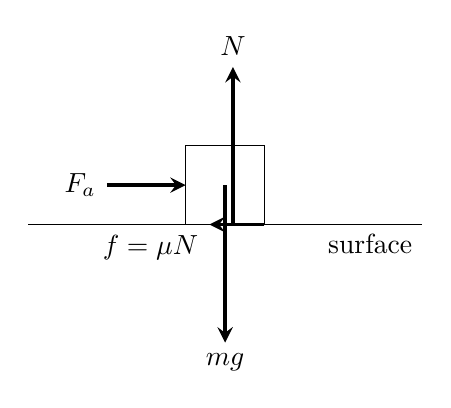
\begin{tikzpicture}
				\draw (2,0) -- (2,1) -- (3,1) -- (3,0);
				\draw [line width=0.5mm, -stealth] (2.5,0.5) -- (2.5,-1.5) node[anchor=north] {\(mg\)};
				\draw [line width=0.5mm, -stealth] (2.6,0) -- (2.6,2) node[anchor=south] {\(N\)};
				\draw [line width=0.5mm, -stealth] (1,0.5) node[anchor=east] {\(F_a\)} -- (2,0.5);
				\draw [line width=0.5mm, -stealth] (3,0) -- (2.3,0) node[anchor=north east] {\(f = \mu N\)}; 
				\draw (0,0) -- (5,0) node[pos=1.0, anchor=north east] {surface};
				\end{tikzpicture}
			\end{center}
		
			\subsubsection{Centripetal Force}
			\pdef{Centripetal Force}{\textit{(It's not really in syllabus but you need to know this is a thing.)} A centripetal force accelerates a body by changing the direction of the body’s velocity without changing the body’s speed.}
			
			This force arises in uniform circular motion. Centripetal force ``pulls'' the object back to the centre, allowing it to constantly change direction. Centripetal force can be the force of a string pulling a rotating object or a planet orbiting around a star.
			\begin{center}
				\begin{tikzpicture}
				\draw[dashed] (0,0) circle (3cm);
				\draw[line width=0.5mm, -stealth] ({3*sin{30}}, {3*cos{30}}) -- ({1.5*sin{30}}, {1.5*cos{30}}) node[anchor=south east]{\(F_C\)};
				\draw[line width=0.5mm] ({3*sin{30}}, {3*cos{30}}) -- (0,0);
				\fill (0,0) circle (0.5mm);
				\fill ({3*sin{30}}, {3*cos{30}}) circle (2mm);
				\draw[line width=0.25mm, -stealth] ({3*sin{30}}, {3*cos{30}}) -- ++(330:1.5) node[pos=0.5, anchor=south west]{\(v_\mathrm{tangential}\)};
				\end{tikzpicture}
			\end{center}
		
			\[F_C = \frac{mv_\mathrm{tangential}^2}{r} \]
			
			The magnitude of \(v_\mathrm{tangential}\) stays constant, but the direction is constantly changing. That means the object is accelerating. This acceleration is called centripetal acceleration.
\end{document}